\documentclass{article}
\usepackage[utf8]{inputenc}
\usepackage[ukrainian]{babel}
\PassOptionsToPackage{hyphens}{url}\usepackage{hyperref}
\title{Прикладні алгоритми. Завдання 1, звіт}
\author{Михайло Голуб}
\usepackage{graphicx}
\graphicspath{ {./img/} }
\begin{document}
\maketitle
\newpage
\textbf{Реалізація класу множина з сортуванням:}
\\\indent

Для реалізації елементу множини на мові програмування Python створено клас \textit{Node}, що містить значення \textit{value} та \textit{next\_node}. Перше містить значення елементу множини, інше вказівник на наступний \textit{Node} (або \textit{None} якщо наступного \textit{Node} немає).\\\indent
Для реалізації множини створено клас \textit{Set}, що містить значення \textit{first\_node} та методи для операцій над собою: \textit{insert, \_\_str\_\_, delete, search, clear, \_\_len\_\_, to\_list}; та іншим представником класу: \textit{union, intersection, set\_difference, sym\_difference}.
\\\\\indent


\textbf{Реалізація методів класу \textit{Set}:}
\\\indent

\textbf{\textit{insert}} -- цей метод додає значення до множини за наступним алгоритмом роботи:
\begin{enumerate}
\item Якщо не існує першого елемента -- створити його та записати туди значення, завершити;
\item Якщо значення нового елемента менше значення першого елемента -- створити новий елемент,зробити новий елемент першим, перший -- другим, завершити;
\item Якщо значення нового елемента рівне першому -- завершити;
\item Крокувати через усі елементи множини: якщо обраний елемент не існує -- вставити новий елемент, завершити; якщо обраний елемент менше обраного -- крокувати далі; якщо обраний елемент більше обраного -- вставити новий елемент перед ним, завершити; якщо обраний та новий елемент мають однакове значення -- завершити.
\end{enumerate}
Кроки 1-3 є частковим випадком 4, оскільки крокування можливо почати лише з 2го елементу не ускладнюючи код циклу.\\\indent

\textbf{\textit{\_\_str\_\_}} -- цей метод крокує через усі елементи множини, записує їх у \textit{list}, потім переганяє їх у \textit{str} та повертає отраману строку.\\\indent
\textbf{\textit{to list}} -- цей метод крокує через усі елементи множини, записує їх у \textit{list} та повертає його.\\\indent

\textbf{\textit{delete}} -- цей метод видаляє значення з множини за наступним алгоритмом роботи:
\begin{enumerate}
\item Якщо множина пуста -- завершити;
\item Якщо значення менше першого елемента -- завершити;
\item Якщо значення рівне першому елементу -- видалити його, зробити другий елемент першим, завершити;
\item Крокувати через усі елементи множини: якщо обраний елемент не існує -- завершити; якщо значення рівне значенню обраного елемента -- видалити його, зв'язати сусідні елементи між собою, завершити; інакше -- крокувати далі.
\end{enumerate}\indent

\textbf{\textit{search}} -- цей метод перевіряє наявність елемента в множині за наступним алгоритмом роботи:
\begin{enumerate}
\item Якщо множина пуста -- повернути -1;
\item Якщо значення менше першого елемента -- повернути -1;
\item Якщо значення рівне першому елементу -- повернути 0;
\item Крокувати через усі елементи множини: якщо обраний елемент не існує -- повернути -1; якщо значення рівне значенню обраного елемента -- повернути його позицію; інакше -- крокувати далі.
\end{enumerate}\indent

\textbf{\textit{clear}} -- цей метод видаляє відв'язує перший елемент від множини, після чого його десь там підбирає garbage collector.\\\\\indent
Бінарні методи класу множини реалізовані за загальним принципом:
\begin{enumerate}
\item Виконати відповідну дію якщо одна або обидві з множин пусті
\item Крокувати через обидві множини: порівнювати обрані елементи, якщо виконується умова операції -- виконати дію; інакше -- зробити крок в множині чий обраний елемент менший
\end{enumerate}
Детальний опис цих методів займе більше часу ніж усе інше сумарно, тому він буде пропущений.
\\\\\indent

\pagebreak
\textbf{Тестування швидкості роботи:}
\\\indent

Дядько Фестер (Аддамс), представник класу \textit{SkilledTester}, проводить тестування наступним чином: отримує два "синхронізовані" масиви: "потужність множин" та "кількість тестувань"; тестує, та повертає масив середніх часів виконання. Після цього створюється графік залежності часу виконання (в мкс) від потужності множини.\\\indent
Результати тестування \textit{search} елементів яких немає в множині:
\begin{center}
    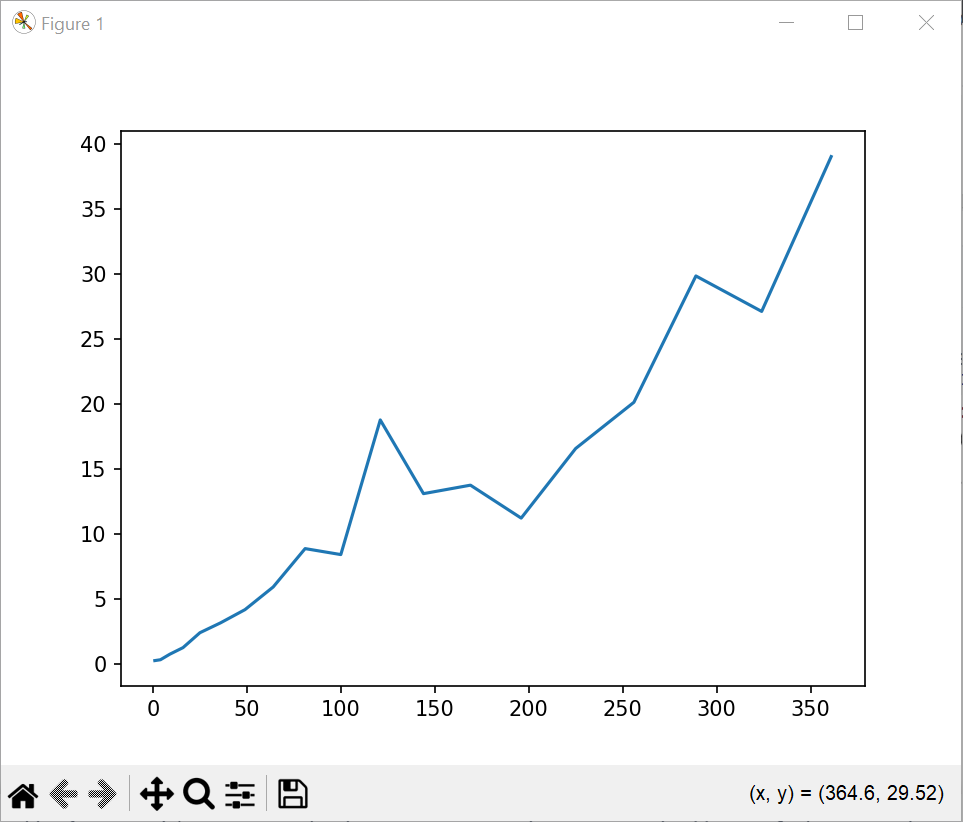
\includegraphics[width=125mm]{search}
\end{center}

Протестовано 19 вибірок потужністю від 1 до 361. Не дивлячись на малу кількість точок та значне коливання значень, видно що залежність часу виконання від потужності схожа на лінійну функцію. Це очікувано, оскільку алгоритм не має вкладених циклів і в середньому має складність O($\frac{n}{2}$)\\\indent

Результати тестування \textit{search} елементів які є в множині:\\\indent

\begin{center}
    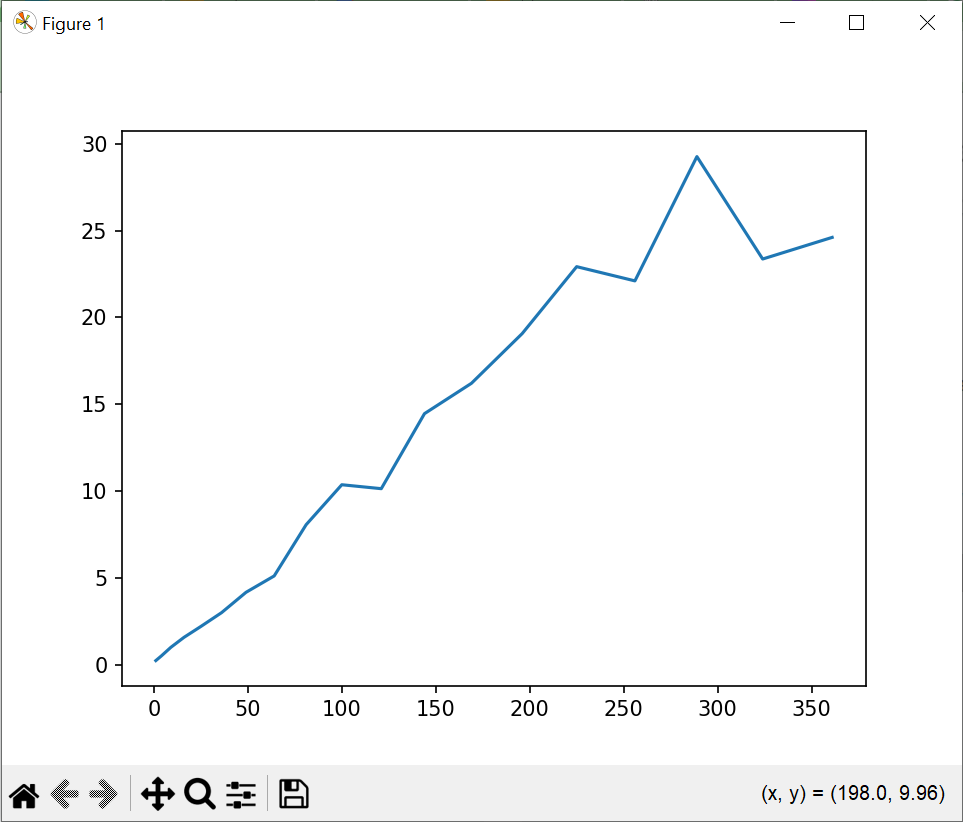
\includegraphics[width=125mm]{search_for_element}
\end{center}

Протестовано 19 вибірок потужністю від 1 до 361. Не дивлячись на малу кількість точок та значне коливання значень, видно що залежність часу виконання від потужності схожа на лінійну функцію. Це очікувано, оскільку алгоритм не має вкладених циклів і в середньому має складність O($\frac{n}{2}$)\\\indent

Результати тестування \textit{union} множин:\\\indent

\begin{center}
    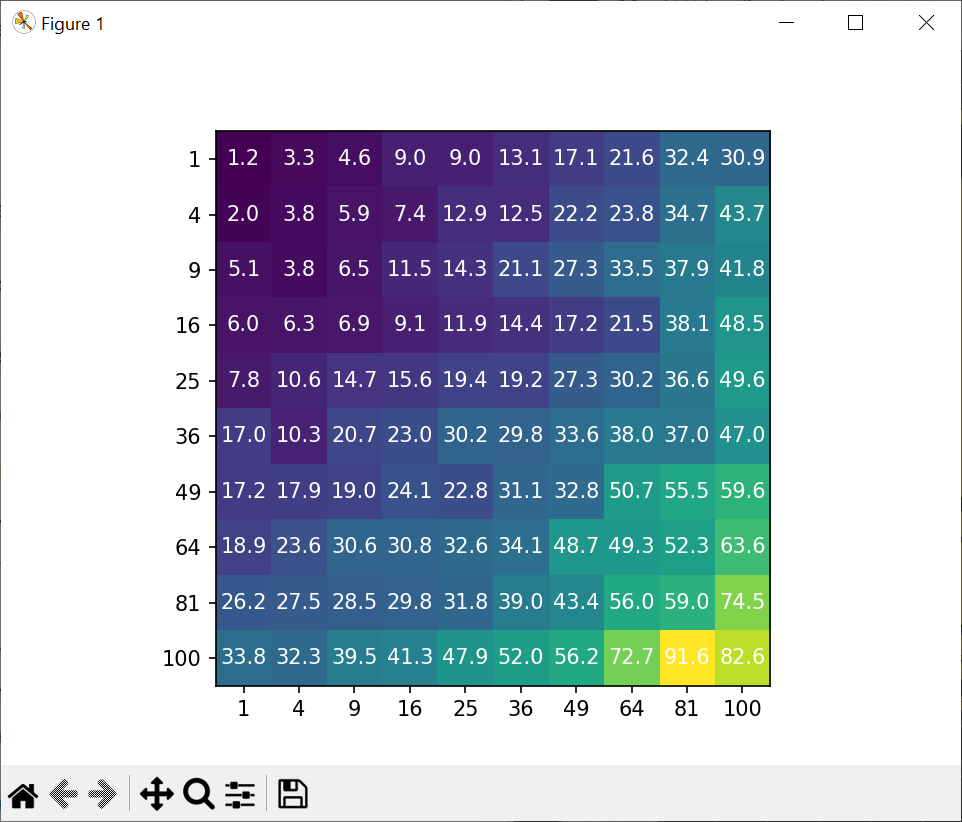
\includegraphics[width=125mm]{union}
\end{center}

Протестовано 100 пар вибірок множин потужністю від 1 до 100. З heatmap видно, що збільшення сумарної кількості елементів множин в 2 рази призводить збільшення часу в 1.7-2.5 рази. Це очікувано, оскільки алгоритм не може зробити ітерацій більше ніж є сумарно елементів у множинах, а отже має найгіршу складність O($n_1 + n_2$)\\\\\indent

Посилання на репозиторій практикуму:\\ \href{$https://github.com/MINIAProgramStudio/applied_algorythms/tree/main/task_1$}{$https://github.com/MINIAProgramStudio/applied\_algorythms/tree/main/task\_1$}\sloppy

   
\end{document}